\documentclass[11pt,a4paper]{report}

% Aberstwyth dissertation LaTeX Template
% Authors: Dr. Hannah Dee (hmd1@aber.ac.uk), Neil Taylor (nst@aber.ac.uk)
% This has been adapted from the Leeds Thesis template and the 
% Group Project template for Computer Science in Aberystywth University.
% 
% All comments and suggestions welcome.
%
% Template designed to be used with pdflatex: it may need alteration to
% run with a different LaTeX engine.
%
% Note - this is offered as a starting point for your work. You are not 
% required to use this template and can choose to create your own document 
% without it. 

% To build document on the unix command line, run four commands:
 
% pdflatex dissertation
% bibtex dissertation
% pdflatex dissertation
% pdflatex dissertation

% you will end up with dissertation.pdf 
\usepackage{mmp}

% the following packages are used for citations - You only need to include one. 
%
% Use the cite package if you are using the numeric style (e.g. IEEEannot). 
% Use the natbib package if you are using the author-date style (e.g. authordate2annot). 
% Only use one of these and comment out the other one. 
\usepackage{cite}
%\usepackage{natbib}

\usepackage{graphicx}
\usepackage{rotating}

% Use the following to selectively exclude chapters
%\includeonly{cover,abstract,acknowledge,declare,chapter1,chapter2}

\begin{document}

% all of the include directives below refer to tex files
% so 
\title{Classroom Quiz System}

% Your name
\author{Alexander Taylor}

% Your email 
\authoremail{amt22@aber.ac.uk}

\degreeschemecode{G401} %e.g. G400 
\degreeschemetitle{TODO: Computer Science With A Year In Industry} % e.g. Computer Science
\degreetype{BSc}

\modulecode{CS39440} % i.e. CS39440, CC39440, CS39620
\moduletitle{Major Project} % i.e. Major Project or Minor Project

\date{13th April 2017} % i.e. the date of this version of the report

\status{Draft} % Use draft until you create the release version. Then, change this to Release.
\version{1.1}

%The title and name of your supervisor.
\supervisor{Mr. Chris Loftus} 

%The email for your supervisor. 
\supervisoremail{cwl@aber.ac.uk}

\maketitle



 includes cover.tex - to change the content,
% edit the tex file

\pagenumbering{roman}

% This is the front page

\title{Classroom Quiz System}

% Your name
\author{Alexander Taylor}

% Your email 
\authoremail{amt22@aber.ac.uk}

\degreeschemecode{G401} %e.g. G400 
\degreeschemetitle{TODO: Computer Science With A Year In Industry} % e.g. Computer Science
\degreetype{BSc}

\modulecode{CS39440} % i.e. CS39440, CC39440, CS39620
\moduletitle{Major Project} % i.e. Major Project or Minor Project

\date{13th April 2017} % i.e. the date of this version of the report

\status{Draft} % Use draft until you create the release version. Then, change this to Release.
\version{1.1}

%The title and name of your supervisor.
\supervisor{Mr. Chris Loftus} 

%The email for your supervisor. 
\supervisoremail{cwl@aber.ac.uk}

\maketitle



                        

% Set up page numbering
\pagestyle{empty}

% declarations of originality 
\thispagestyle{empty}

%%%
%%% You must sign the declaration of originality. 
%%%
\begin{center}
    {\LARGE\bf Declaration of originality}
\end{center}

I confirm that:

\begin{itemize}
\item{This submission is my own work, except where 
clearly indicated.}

\item{I understand that there are severe penalties for Unacceptable Academic Practice, which can lead to loss of marks or even the withholding of a degree.}
 
\item{I have read the regulations on Unacceptable Academic Practice from the University's Academic Quality and Records Office (AQRO) and the relevant sections of the current Student Handbook of the Department of Computer Science.}
 
\item{In submitting this work I understand and agree to abide by the University's regulations governing these issues.}
\end{itemize}

\vspace{2em}
Name ............................................................  \\

\vspace{1em}
Date ............................................................ \\

%%% 
%%% We would like to make a selection of final reports available to students that take 
%%% this module in future years. To enable us to do this, we require your consent. You 
%%% are not required that you do this, but if you do give your consent, then we will have 
%%% the option to select yours as one of a number of reports as examples for other 
%%% students. If you would like to give your consent, then please include the following 
%%% text and sign below. 
%%% 
%%% If you do not wish to give your consent, please remove this from your report. 
%%%
\vspace{1em}
\begin{center}
    {\LARGE\bf Consent to share this work}
\end{center}

By including my name below, I hereby agree to this dissertation being made available to other
students and academic staff of the Aberystwyth Computer Science Department.  

\vspace{2em}
Name ............................................................  \\

\vspace{1em}
Date ............................................................ \\


               

\thispagestyle{empty}

\begin{center}
    {\LARGE\bf Acknowledgements}
\end{center}

I'd like to thank my supervisor Chris Loftus for his continuous support and advice throughout the project, and my second marker Laurence Tyler for his feedback from the mid project demonstration. In addition, I would like to thank Alun Jones, Stephen James and Max Atkins for helping set me up a server to use for hosting the project.

I am also grateful to Carly Jackson and Kerey Taylor for taking time out to proof read my dissertation.
 % Acknowledgements
\thispagestyle{empty}

\begin{center}
    {\LARGE\bf Abstract}
\end{center}

The focus of this project was to create an application that can be used by lecturers to allow students to answer questions and display these results live in lectures. The project was based on a pre-existing application, called Qwizdom\cite{Qwizdom} but this project aims to improve upon Qwizdom in several ways.

The system is a web based application built in Laravel, a PHP based framework. The system provides two main functions, the running of questions on their own, and streaming lecture slides with questions embedded within the slides to students. This system improves upon Qwizdom in several ways. Firstly, it runs via a website rather than via a PowerPoint extension, meaning more lecturers can use it. Furthermore, it provides more functionality such as more possible answers and students cannot submit their own answers as they can with Qwizdom.

Development followed an Extreme Programming approach, utilising a number of practices to help development. Stories were created and used as the functional requirements for the system, and stories were worked on individually within weekly iterations. Analysis, design, implementation and testing were done for each story rather than having an upfront design stage or end testing stage.

TODO: mention user testing when thats done

TODO: summary of eval when written?                 % Abstract

\pagenumbering{roman}
\pagestyle{fancy}
\fancyhead{}
\fancyfoot[C]{\thepage}
\renewcommand{\headrulewidth}{0 pt}
\renewcommand{\chaptermark}[1]{\markboth{#1}{}}

\tableofcontents   
\newpage
\listoffigures
\newpage 
\listoftables
\newpage

% Set up page numbering
\pagenumbering{arabic}

\setchapterheaderfooter

% include the chapters
\chapter{Background \& Objectives}
\section{Background} 
\subsection{Qwizdom}
Currently lecturers at Aberystwyth University have the option to use a service called Qwizdom\cite{Qwizdom} which allows lecturers to embed quiz questions into their slideshow presentations. During a lecture, students can join a session through an online portal and have the slides and questions streamed through to their devices. Quiz questions can then be answered by the students and their results can be displayed live by the lecturer, who can also save these results for later analysis.

\subsection{Replacement}
A replacement system was wanted to fix some of the problems that Qwizdom has. Primarily that the university only has one session key, which means only one session can be used by all lecturers at any one time, leading to some clashes. With a new system, there would be no limit to the number of sessions that can be run. Other problems with Qwizdom include:
\begin{itemize}
	\item Maximum of 6 answers
	\item Students can submit their own answers by changing the HTML on the page
	\item Creating quizzes is tied into Microsoft PowerPoint which not all lecturers use
	\item Ageing interface on the student end
\end{itemize}

\section{Analysis}
\subsection{Two parts}
It was decided that the project would be split into two main parts, the first was to create an application that lecturers can run a simple quiz from without any slides. The second part involves developing an application or extension to the first part that allows the lecturer to create the quiz as part of a set of slides. The slide the lecturer is viewing would then be displayed in the quiz session on the web where students can access it. Once a relevant quiz slide appears, the students will be given the quiz options to select an answer in the same way as the first part. The lecturer can then display the results in the same way, though it would not be via the web application as before. This part of the project behaves in much the same was as Qwizdom.
The reason for having two parts is that the first would be mostly built as part of the development for the second part but if built as a standalone part it allows lecturers to create quizzes rather than a set of slides with quizzes within it. Features like the session joining, front-end view for students and the way answers are submitted would be used in the second part, which means only creating quizzes would need to be added for the first part for it to be stand alone. Additionally, the second part had the potential to be much larger in scope than originally anticipated and as such having the first part to extend in a different direction should the second part become unviable would be provide a safety net.

\subsection{Part 1}
A web based approach was chosen for the first part. This application would allow lecturers to log in to an admin panel and from there create and run quizzes for the students. This would also lay the groundwork for the second part, setting up the front end for students, how sessions are run and how answering questions worked. 
\subsubsection{Framework}
PHP was the language selected due to two primary reasons. The first is that the developer was familiar with PHP after using it in an industrial job. The second is that a large number of University projects are PHP based which will make integrating this with the University easier in the future. Whilst Ruby or Javascript might be applicable, the familiarity and ability to extend PHP made it the best choice.
\subsubsection{Laravel}
Laravel is a web framework written in PHP, and has been chosen for the web server part of this project\cite{laravel}. There are a number of reasons for choosing Laravel in this project over other available frameworks. The first and most important is familiarity with Laravel as the developer has used it in the past, and the main framework used in their year in industry was based on Laravel.

Laravel is also the most popular PHP framework available\cite{PopularPHPFrameworks}, which means there is an enormous amount of support available in the form of user forums, video guides and its own tag on Stack Overflow.

Laravel 5 also natively supports WebSockets, a technology that was being considered for the first part of the project. Other features of Laravel is its conformance to PSR-2, a PHP coding standard, meaning it would be easier to follow good coding standards more easily.
\subsection{Part 2}
The second part required more extensive research to be done when it was reached in development. But the main suggestion was to create a Microsoft PowerPoint extension much like Qwizdom to create slides embedded with questions\cite{powerpoint-addins}. Due to the size of such an undertaking, another potential solution was to create the web application in such a way that an extension could be worked on in the future, i.e. set up the system for future extensions.
\newpage

\section{Process}
The methodology chosen for this project was an Extreme Programming (XP) based approach. One of the core advantages of using an XP based approach is the ability to adapt to change. The second part of this project, implementing a method to stream slides to students, was much more open to change than the first part where the scope was far more understood. If another process such as Feature Driven Development was used, it would work for the first part of the project as all the requirements and features are known but most likely would be a struggle to use in the second part. XP gives the flexibility needed to complete the second part of the project whilst also allowing the first part to be done with ease.

\subsection{Practices}
XP does not enforce the use of any single practice and as such a number of practices were selected for the project that work in a single developer project:
\begin{itemize}
	\item Test Driven Development - Writing tests before coding any of the application logic helps to enhance both the design and also mean tests should actually be written rather than left until the end and "hacked" in.
	\item Coding Standards - Keeping to strict coding standards helps ensure the code is good quality and easy to extend in the future as this project may well be.
	\item Small Releases - Small releases help enforce releases bit of working code regularly and results in a better overall project if the sub parts are all working.
	\item On Site Customer - This practice is somewhat applicable, the developer can act as a customer, and the project supervisor can also somewhat act as a customer, due to them being the originator of the idea and also a lecturer, one of the main users of this application.
	\item Merciless Refactoring - Refactoring is already encouraged by using TDD, but it can also be used at other points in the project to ensure the code is structured sensibly.
	\item Planning Game - This can be adapted to be done by one person at the start of the project, the list of stories was written and then iterations and releases planned out.
	\item Continuous Integration - Some online tools can be used to provide an CI workflow, to run tests continually with the constant small releases.
\end{itemize}

On the flip side, a number of practices were less appropriate and had to be dropped, such as Pair Programming and Collective Code Ownership, due to there only being one developer.

\subsection{Stories - functional requirements}
Before any development could start, an initial list of functional requirements was needed. For an XP based project, these would be in the form of "stories". The stories have a difficulty ranking associated with each item in relation to the other stories. 1 would the easiest and 10 the hardest. See appendix \ref{appendix:stories}.1 for the intial list of user stories.

\section{Planning Game}
A plan was created early in development:
\begin{itemize}
	\item 10 iterations beginning on Thursdays remaining from when the original plan was made (22/02/2017)
	\item Leave 2 iterations for Report Writing and emergency bug fixing at the end, from iterations beginning 20/04/2017
	\item 8 iterations between planning and iteration 8, these to be devoted to majority of coding
	\item ~3 iterations before mid-project demonstration from initial planning
\end{itemize}
It was decided that it would be beneficial to try and get the majority of coding done within the 8 iterations specified, this would give the final two iterations breathing room to put together the final document more formally and give some bug fixing time and cleaning up time. In terms of releases, the aim was to have sets of features that would be releasable at the end of every iteration, though no planning of which features being released when was made.
\newpage
%\addcontentsline{toc}{chapter}{Development Process}
\chapter{Design}
This chapter will give an overview of the design of the final system, however will not go into much detail for individual parts of the system. Those designs are within the next chapter as design took place within each iteration rather than at the start.
TODO: could this chapter actually be after the Iteration chapter, might make more sense?

\section{Overall Architecture}
The Laravel framework uses a Model-View-Controller design pattern to build applications. It works in the same way as a normal MVC application. Data is stored and manipulated within the models, controllers handle most of the interactions the user has with the system, and the views are the web pages presented to the users. Within Laravel, there is also a front controller, which is used to route incoming HTTP requests to the appropriate views and controllers\cite{Laravel-architechture}.

There are two basic sections of the system, the student end, and the lecturer end. The lecturer end is an admin panel that they can login to, to create and manage their quizzes. The student end consists of the portal for connecting to a session, and the session pages themselves that display the slides and questions for users to answer.

Students only have two bits of functionality available to  them, being able to join a quiz and then being able to answer questions. Lecturers however can do much more on the site. On the admin panel they can create new quizzes, create and add questions to the quizzes and also add slides to the quizzes. They can also change their user details including their session key. The main operation they can perform is that they can run a quiz, this then takes them to the same view as the students, albeit with a small control panel for changing questions or slides, and displaying the results of the quiz.

\section{Database Design}
\begin{sidewaysfigure}
	\caption{Entity relationship digram for final database}
	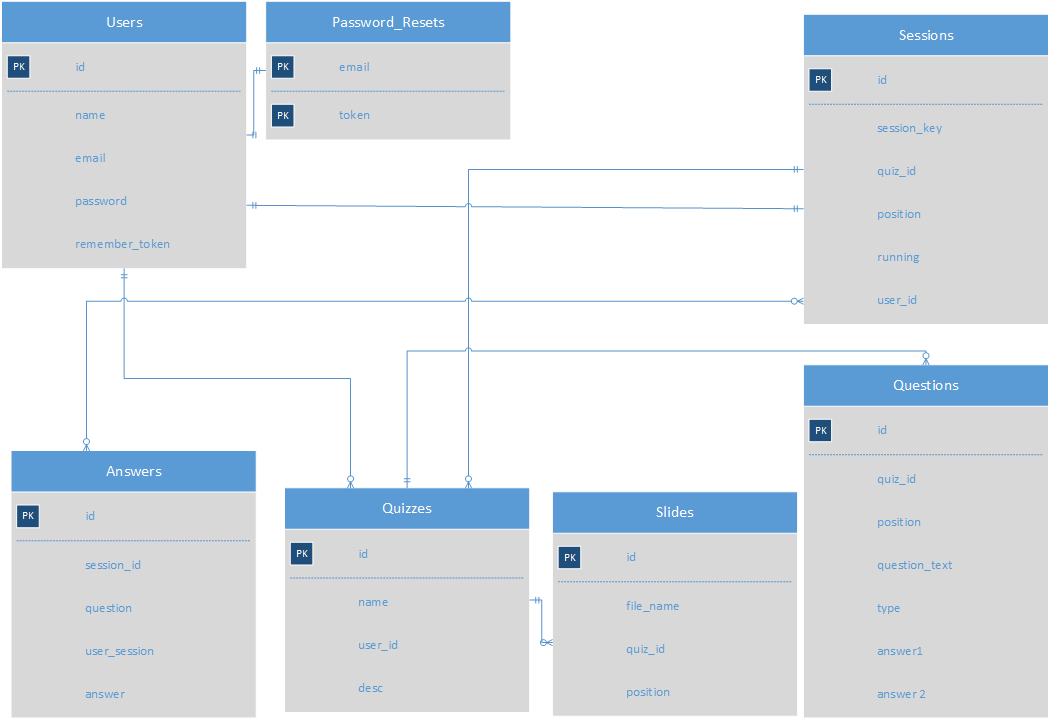
\includegraphics[width=\textwidth]{Chapter2/Final-ER-Image}
	\label{fig:er-diagram}
\end{sidewaysfigure}
\newpage

There are seven tables within the application. Two of these were generated by running a Laravel command to make the authentication part of the site, the users and password\_resets tables. These provide basic user login.

The quizzes table contains information about the quizzes themselves, and are associated with a user. The questions and slides tables both store information about their respective parts of a quiz, with each row within these tables associated with a quiz. Questions store information about the actual question including all the answers, not in the design above are the other eight fields for answers up to answer10. The slides table stores the file name of a slide image that has been converted from a pdf slide. Both of these tables store the positions of their items within a quiz.

The sessions table stores the information about the runnable session, each user has one associated session row. Within this row, the session\_key is stored, which is the key that students would use to connect to a session. Additionally it stores information about the session when its running, specifying if it is running, and what position it is at. This position references the positions specified int he questions and slides tables, though there is no actual foreign key relationship between them. 

The final table, answers, stores all the responses from users to questions. It stores which question, the answer given and the user that submitted the answer. The user\_session is a cookie value rather than a user from the database.
\chapter{Iterations}
\section{Tools used}
There were a number of tools used throughout development that do not fit under a single iteration. The main three were a Wordpress diary, a Trello board and Git. 

The diary was used to keep track of the major pieces of development done each week and any questions/ issues that needed to be raised during supervisor meetings. This was a simple Wordpress site that was set up several years ago and repurposed for the use in this project.

Trello is a project management tool that allows users to create a "board" for a project that then allows the creation of cards that tasks can be added to\cite{trello}. Feature tracking is a key part of the system as tasks and cards can be marked as complete, Trello suits XP based approaches as cards can be created and edited on the fly for each iteration. For this project, a card was created for each iteration, with a list of stories and tasks to be completed within that iteration. Once a task was completed, it was checked as such giving an easy to read percentage completion for the story.

Git was used extensively during development, primarily for version control but also a form of backup and as an easy way to deploy the system. Version control is very important as it allows tracking changes to the project and if a mistake it made, can be used to undo these mistakes. It also allows branching out bits of functionality, so developing features can be done separate from the rest of the project and once working, merged back in. Github was used as the repository service due to it being free and easy to use\cite{github}.
\newpage

\section{Iteration 0 16/02 - 22/02}
\subsection{Initial work}
This iteration did not consist of any development. It consisted mainly of research and design work. But most importantly it included writing the stories for the project. 

Other items of work involved setting up a diary, a Trello board for documenting all the work and setting up the initial Git repository along with linking it to Github.
\subsubsection{Research}
Research was focussed on several areas, and some documents were produced from this research. The first area of research was on the frameworks available, after which Laravel was selected. Hosting options were also explored and a document discussing both of these was produced, this document will form part of the Background chapter when it comes to writing the report.

Some additional research was also completed on the Microsoft PowerPoint Add-In for the second part of the project. This was mainly to get a sense of the amount of work involved, and what language/ environments would be needed. This research did not go into much depth as further research will be undertaken when that part of the work is reached.
\subsubsection{Design}
The design work completed was a database design. This would be needed throughout the whole project so made sense to write initially, though it may be subject to significant changes. Figure \ref{fig:initial-er-diagram} is the ER diagram.

\begin{sidewaysfigure}
	\caption{Entity relationship digram for the initial database}
	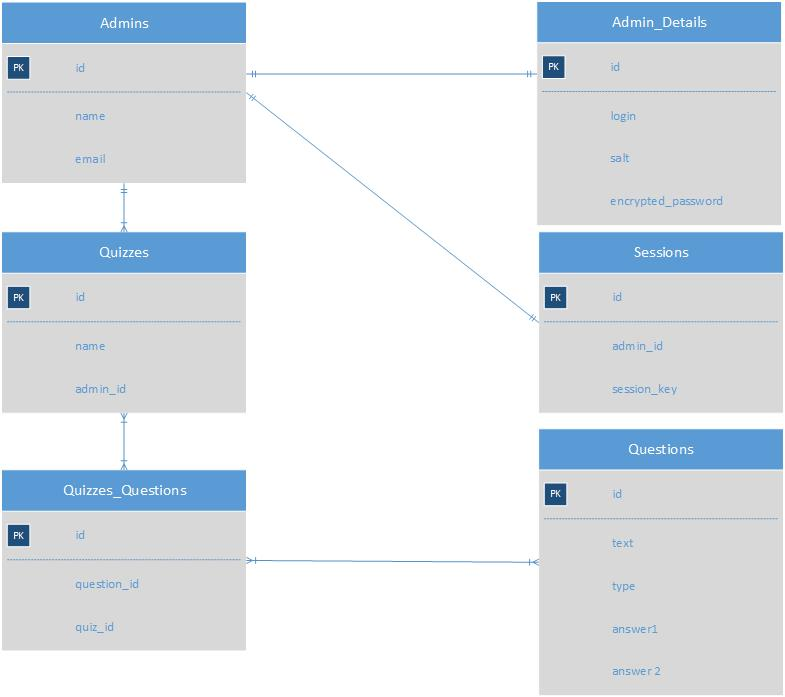
\includegraphics[width=\textwidth]{Chapter2/Iter-0/Initial-ERDiagram}
	\label{fig:initial-er-diagram}
\end{sidewaysfigure}

\subsubsection{Stories}
A list of stories was produced and written up in a separate document. These stories will be the basis of the project and act as the functional requirements for the evaluation at the end of development (appendix \ref{appendix:initial-stories}).
\newpage

\section{Iteration 1 23/02 - 01/03}
\subsection{Story: Admins can create quizzes via the website}
\subsubsection{Analysis - Breakdown of Tasks}
This story is quite large and should be broken down into several substories:
\begin{itemize}
	\item (3) Admins can log into a backend
	\item (2) They are presented a list of their quizzes
	\item (5) They can create a new quiz in the backend
	\item (3) They can edit an existing quiz they own
\end{itemize}
These have been added to the story list document.
\newpage

\subsection{Story: Admins can log into the backend}
\subsubsection{Analysis - Breakdown of Tasks}
\begin{itemize}
	\item Create users table
	\item Add login page
	\item Add register page
\end{itemize}
\subsubsection{Design}
Design was limited due to the automated builder. However it added some view files and a default HomeController for a basic homepage.
\subsubsection{Implementation}
Implementing this was far easier than originally anticipated, Laravel comes with the needed tables out of the box and has a command to run that sets up simple auth for users: \textit{php artisan make:auth}
\subsubsection{Testing}
Because the login and auth is handled by Laravel by default, testing it was deemed to not be a priority. However, three simple tests were written to ensure it never breaks due to future changes. Dusk Tests:
\begin{enumerate}
	\item Test to ensure the application redirects to /login is the user is not already logged in
	\item Test for logging in with a user in the database
	\item Test for registering a new user
\end{enumerate}
\newpage

\subsection{Story: They are presented a list of their quizzes}
\subsubsection{Analysis - Breakdown of Tasks}
\begin{itemize}
	\item Make the homepage the QuizController rather than the HomeController
	\item Check and get the user who is logged in
	\item Display a list of quizzes for that user
\end{itemize}
\subsubsection{Design}
The HomeController to be removed in this period of work and the QuizController used in its place. (TODO: Digitize UI mock)
\subsubsection{Implementation}
Quite an easy amount of work, changing the controller was a simple change to the routes and then updating the quiz view file to use the same layout as the original home views. To get the user, a helper function is provided: \textit{auth()-$>$user()} which gets the user object. Obtaining the id from this is simple and then using an Eloquent ORM call it is easy to find all the quizzes owned by that user.
\subsubsection{Testing}
Dusk tests for this story:
\begin{enumerate}
	\item Test to see if the /home page lists the quizzes as it would on the /quizzes page
	\item Test to see if a quiz that belongs to a user is present on the page
	\item Test to see if a quiz that belongs to another user is not present on your page whilst your own is
\end{enumerate}
These tests highlighted a problem with the testing framework however. Chrome is used as the Remote Web Driver for running these application tests in. For each test a new migration is made within the test database, thereby wiping the data created within each test. An unintended side effect however is that every new user created starts at id=1 in the users table (a user has to be created for all these tests.) The Chrome driver seems to remember that the user of id=1 logged in, in the previous test and therefore skips the auth step. This means the test order is messed up due to the test trying to log in even though it is already logged in. The solution to this is to create each new user in the next id record, whilst this is somewhat convoluted, it seems to work.

Potential future tests: Use sessions have two users log in and see/ not see the relevant quizzes.
\newpage

\subsection{Non-Story Work}
\subsubsection{Database Work}
Some initial work that is needed for almost all the stories is having a working database set up to store the users, quizzes, questions etc. Seeing as the amount of work to setup all the tables and their relationships would not take long, it was decided that this could be done all at once at the start of the iteration.

While creating these tables it was possible to create the controllers needed within the application at the same time using: \textit{php artisan make:model *name* -mc } 
\subsubsection{Seed Data}
Because of the amount of changes to the database that were being made, the tables were repeatedly wiped and seeding some data was needed. To do this some seeders were generated with \textit{php artisan make: seed *name*}. These were created under database/seeds/ and simply required creating new objects of the desired Model and adding the various fields as parameters of the objects. These objects are then saved to the database. These seeders can be run when a migration is called such that the data is replaced as soon as its lost.
\subsubsection{Layout Changes}
The initial \textit{make:auth} command created a default home page with a menu bar and some basic styling. This styling was created with Bootstrap and looks quite nice so the basic styling has been kept. This layout was modified somewhat to add some menu options that persist across pages. This layout is then used by all the backend pages created by extending it.
\newpage


\section{Iteration 2 02/03 - 08/03}
\subsection{Story: They can create a new quiz in the backend}
\subsubsection{Analysis - Breakdown of Tasks}
\begin{itemize}
	\item Need quiz/new form to add name
	\item Add validation
	\item This then redirects to quiz.show for this new quiz
	\item This page needs a button that can add a question
\end{itemize}
\subsubsection{Design}
The design is split into two parts, design for the quiz/new page and a design for the question/new page:
(TODO: digitise images for these)
Use case at this point \ref{fig:quiz-create-use-case}
\begin{figure}
	\caption{Use case diagram for the admin backend with create quiz functionality}
	\centerline{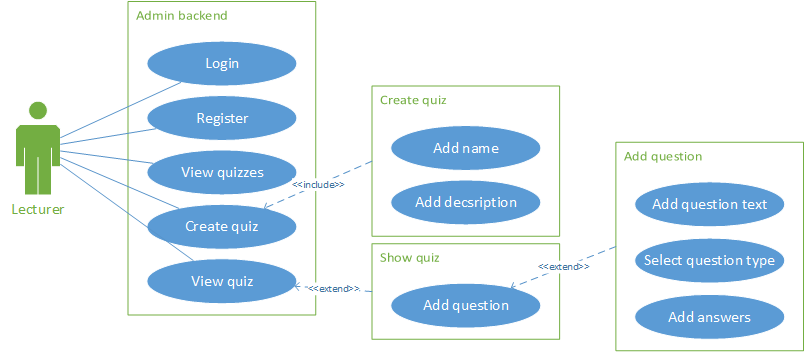
\includegraphics{Chapter2/Iter-2/iter-2-use-case-create}}
	\label{fig:quiz-create-use-case}
\end{figure}
\subsubsection{Implementation}
A create page was added for quizzes, this was linked to from the home page. This was mapped to /quizzes/create address. A simple form was added to this page with the name and description of the quiz. Questions would be added on an individual quiz page. The form sends the form as an HTTP POST request to the /quizzes page which then maps onto the 'Store' action in the Quiz Controller. This action is used for server side validation and saving the data to the database using an Eloquent function. This Eloquent function also returns the id of the new quiz. The user\_id is assigned to the quiz by simply getting the current user. Using this id, this Store function redirects to the newly created quiz.

On a quiz page, it displays the name and description and has a button to add any questions to the quiz. This button links to the questions/create page that functions in the same way as the quiz creation, albeit with the relevant fields in the form. The questions are assigned to the quiz by passing the quiz id to the question creation page in a GET variables via the url. This allows the question to be assigned to the quiz during its creation in the database and to be redirected back to the quiz page.

For validation there are two parts, one on the HTML form and the other handles server side. The HTML validation (client side) uses simple HTML 5 validation like the "required" attribute in the form inputs. Further frontend validation could be added utilising JavaScript but the HTML solution was far easier to implement, being the addition of one word and not several lines of code that have to be built and added to the correct pages. The server side complements this as client side validation can be circumnavigated by determined users.

The server side validation in Laravel is well supported and made as easy as possible to implement. The Store function used to save data from the POST request simply calls \textit{\$this-\textgreater validate()} on the request data. Inside this validation function, various rules can be imposed on individual pieces of the request data such as simply requiring that is is filled or that it has to have a minimum length\cite{laravel-validation}.

Something that Laravel enforces is the use of CSRF tokens to prevent cross site request forgery attacks on the site. A token is generated for the project during its creation, and this token must be placed in a hidden field within every form so that it can verify that the authenticated user is the one actually making the requests to the application\cite{laravel-csrf}.
\subsubsection{Testing}
Dusk tests:
\begin{enumerate}
	\item Test to create a new quiz
	\item Test the HTML validation for creating a new quiz
	\item Test backend validation of quizzes
	\item Test a quiz contains questions that have all been added before hand
	\item Test to add a question to a quiz
	\item Test to make sure the question page contains the relevant information
\end{enumerate}
A problem encountered in this set of tests is the speed of testing. Running these tests takes about a minute. The reason for this is that the tests use DatabaseMigrations rather than DatabaseTransactions, meaning that the database is migrated for every test. Using transactions would reduce the time taken by only doing a migration at the start and then using a transaction for each test. Alternatively having a pre migrated test database on which you run transactions would work too, but this would mean any time you change your database, you would have to remember to migrate the test database. 

After attempting to use the transactions it appears as though they are not usable within Dusk. This is because Dusk is running in another process and migrations is the only choice\cite{dusk-transactions}. 
\newpage

\subsection{Story: They can edit an existing quiz they own}
\subsubsection{Analysis - Breakdown of Tasks}
\begin{itemize}
	\item There is an edit button on quizzes that links to quiz/edit
	\item You can edit the name of the quiz
	\item You can remove questions
	\item You can add questions
	\item You can edit the content of a question
	\item You can delete a quiz and its associated questions
\end{itemize}
\subsubsection{Design}
There was not much design for this stage as it only really adds an edit page which should look the same as the create pages in the above story except that the input fields are pre-filled with data that is being editing. Additionally a delete button should be added for quizzes and questions. (TODO: more design here) Figure \ref{fig:quiz-edit-use-case}
\begin{figure}
	\caption{Use case diagram for the admin backend with edit quiz functionality}
	\centerline{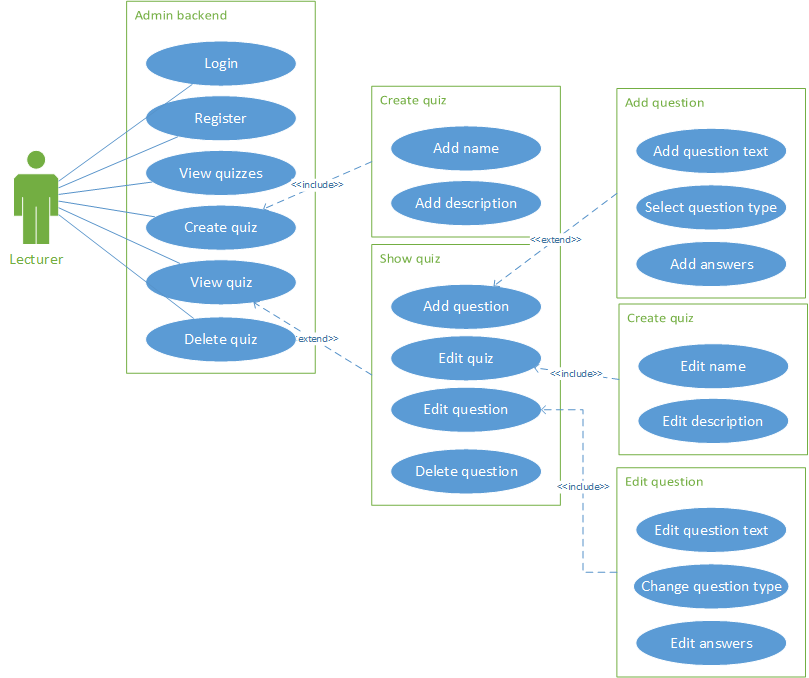
\includegraphics{Chapter2/Iter-2/iter-2-use-case-edit}}
	\label{fig:quiz-edit-use-case}
\end{figure}
\subsubsection{Implementation}
Pre filling the edit page was done by getting the record in the database by the id and just setting the default values of the input fields. The main difference to the creation stage was that the form had to use the HTTP PATCH method rather than POST. This PATCH method is automatically routed to the update function in the controller\cite{laravel-resource-controller}. Within this function, server side validation is performed and and Eloquent called to update the row in the database. It then redirects back to the quiz page for editing either a question or quiz.

Delete buttons were added to the quizzes and questions, these were not a simple \textless a \textgreater tag that linked to a delete page like the create and edit pages. This had to be a small form that sent an HTTP DELETE request along with an id to the /quizzes or /questions page. This was mapped to the destroy functions in the respective controllers which simply called an Eloquent function that removed the record. Due to the way the database is designed when a quiz or question is deleted, the linking row inside the quiz\_question table must also be deleted. 

Another thing that had to be changed was to make the foreign key reference columns in the quizzes and questions table cascade delete on deletion of the record. This meant that they would delete the rows in the quiz\_question table that referenced the row being deleted. For a quiz deletion, this had to go further and also find the questions associated with the quiz and delete all of those, which used a simple Eloquent function to find them using the quiz\_question table before the rows in that table were deleted and then delete the questions using those ids. 
\subsubsection{Testing}
Dusk Tests:
\begin{enumerate}
	\item Test the deletion of a quiz
	\item Test the deletion of a question on a quiz
	\item Test the edit page of a quiz
	\item Test the edit page of a question
\end{enumerate}
\newpage

\subsection{Non-Story Work}
\subsubsection{Seeding}
Some more data needed to be seeded for this subsection of work, the question data. This involved creating some new Model Factories and using them in the seeders correctly. One issue was trying to create many questions for individual quizzes, but this was overcome using some very basic looping and calling the model factories in the right places.
\subsubsection{Quiz Description}
It was decided that quizzes should probably have descriptions attached to them, in case the lecturer needs reminding of what it is in 6 months time. This involved creating a new migration and simply adding a column to the table.
\subsubsection{Travis Setup}
Travis is a CI tool that can be used to run tests automatically on git pushes. Setting it up involved doing some spike work with another git project. It is really easy to set up, needing you to simply add a travis.yml file which specifies what Travis will do after a push. The project also has to be added from Github which is simple.
\newpage


\section{Iteration 3 09/03 - 15/03}
\subsection{Story: Admins can login to the website and run a session with a quiz}
\subsubsection{Analysis - breakdown of tasks}
This story is quite large and whilst it will probably be split into a number of tasks, the first thing to do was some spike work on the way this system would work. One route is with WebSockets, a relatively new technology that allows the server to push data to the page quickly and easily\cite{websockets}. This would be nice solution as it is relatively future proof and seems like a better alternative to other solutions that involve a lot of JavaScript and forcing page changes on the users.
\subsubsection{Design}
WebSockets were introduced into Laravel 5 and have become one of the defacto ways to update the front end in real time. Unlike in some other web frameworks such as Ruby on Rails the web sockets in Laravel requires some extra set up. In Rails the WebSockets can be run on the main web server that is used to run the site\cite{rails-websockets}, in Laravel however another server has to be set up to run these. Laravel offers several different drivers for running the WebSockets, including a Redis server and a third party application called Pusher\cite{laravel-broadcasting}. Pusher handles most of the work for you and requires little set up other than creating a free account\cite{pusher-what-is}.
\subsubsection{Implementation}
Pusher was chosen due to its ease of use and due to its high recommendation rate within the Laravel community. A problem with Pusher is that due to it being a third party service, it is not free forever (it has a number of users limitation). However you could host your own Redis server to mitigate this cost. This means that the system had to be designed in a way that the driver for WebSockets could be changed with ease.

After configuring the spike work application to use Pusher, a simple Laravel Event was created to send a message to the Pusher. To test this event there were a couple methods implemented. The first was to simply register a route that triggers it when the page is visited. (TODO: show an example of an event call?)
 
Or with a custom made artisan command that can trigger the event: php artisan quiz:send {message}. A command is very useful for testing the event as it can be used without building a button on the front end to trigger it.

Two online guides were used to help write this section of the system due to WebSockets being a new technology\cite{pusher-guide}\cite{echo-guide}. Though they were used to get the basic concepts working, the final code used within the project is tailored to the system and is therefore different overall.
\subsubsection{Testing}
There was no testing as it was spike work.
\newpage

\subsection{Non-story work}
\subsubsection{Refactor controllers}
The first major piece of work was to refactor the controllers and models into a far more sensible structure. The problem was that the Eloquent functions for modifying and reading from the database was within the controllers. In a full MVC system, this functionality should be inside the models. To fix this, the Eloquent functions were refactored into the respective quiz and question models. This would make it easier if anything ever needed to change within the logic for any database interactions.
\subsubsection{Changing the DB structure}
The original design was changed, and the quiz\_questions table for linking quizzes and questions together was removed. The original reason for this table was most likely such that questions could be reused. However, after thinking about the potential for that to happen, and the issues that the structure was causing in the model logic it was decided that the quiz\_question table was more of a hindrance than a help.

The questions table now simply has a quiz\_id column that references the quiz it belongs to. Doing this means that the relationships between the two tables are much easier to define in the models, simply having a belongsTo and hasMany function in both that automatically return the necessary data. Thanks to the previous refactoring of model logic, changing this functionality was quite quick. Deleting rows in the database was also simpler now that there was no quiz\_questions table, all the related questions when a quiz is deleted can be deleted at the same time using the onDelete cascade property in the database.
\subsubsection{Front-end setup}
This was the first time that any custom CSS was written and Laravel uses SASS to generate its CSS. To build this SASS into CSS, and also to build any future JavaScript, Laravel Mix was needed to run builds for this code. For this, npm and node had to be installed so that they could run their Webpack build scripts. There were some issues trying to get the build scripts to run, even though it worked on fresh installs of Laravel, but eventually a Github issue was discovered that had some solutions\cite{broken-mix}.
\subsubsection{Dusk and travis}
The aim was to try and set up Laravel Dusk on Travis. Dusk can use a few different browser drivers for running the tests in, by default this is Chrome but Travis comes preconfigured with PhantomJS which is also supported by Dusk. It should be a simple swap in drivers and then to set Travis to run a PhantomJS server. Unfortunately this does not seem to work, and no reason can be found. A supposedly working copy was even cloned and that does not work for therefore it has to be concluded it is currently not working.
\newpage


\section{Iteration 4 16/03 - 22/03}
\subsection{Story: Admins can log into the website and run a session with a quiz}
\subsubsection{Analysis - Breakdown of Tasks}
After doing some spike work last week, this task can now be approached and broken into several sub tasks:
\begin{itemize}
	\item Set up config for Pusher
	\item Add event for broadcasting
	\item Write a command to trigger this event
	\item Add a button to quizzes to trigger this event
	\item Display this on the front end using the JavaScript which listens for Pusher events
	\item Add a session key box to front page
	\item Add session id to users
	\item Allows admins to change their id
	\item When admin clicks run, this id can be entered into the key box to join a channel with the name of the id
	\item The user will be presented with the initial quiz page which will be default filled with the name and description of the quiz
	\item The admin will see the same page but with an "admin panel"
	\item This admin panel has a next and previous button for questions
	\item When these buttons are pressed, the question is sent to pusher
	\item These question are rendered as a form on the user end and admin end
	\item The user can submit the form
\end{itemize}
\subsubsection{Design}
Mockups of the student end of the system: 
\begin{center}
	\begin{figure}
		\caption{Design for a quiz on a desktop}
		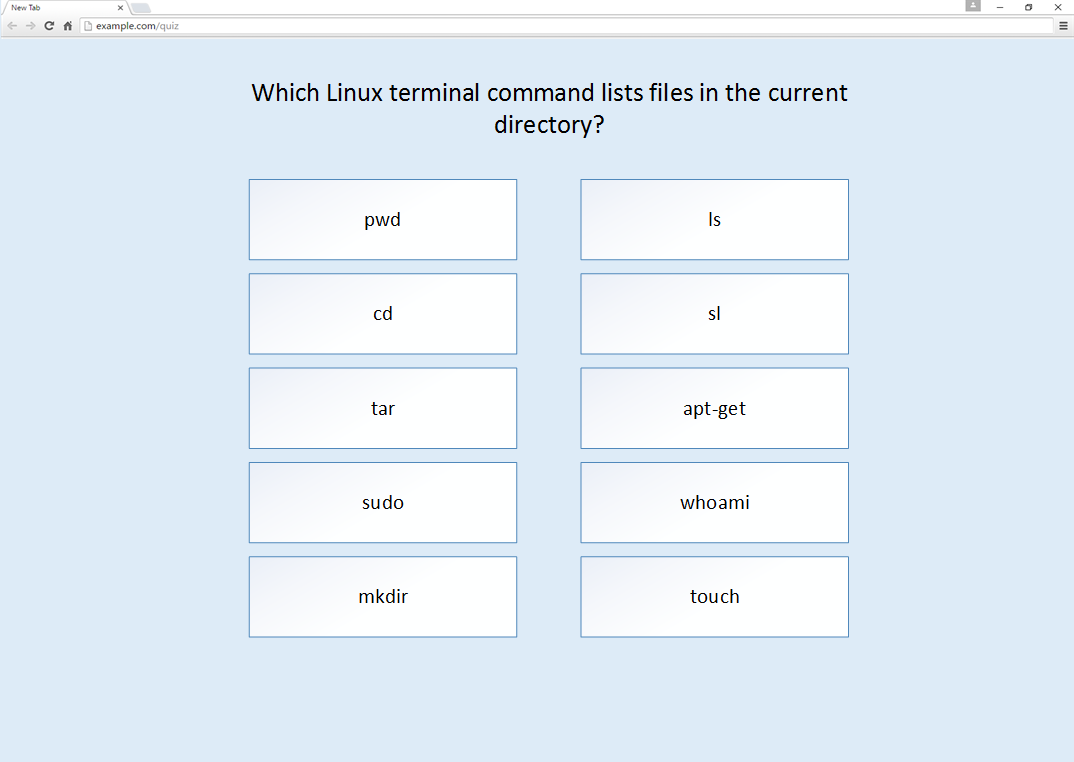
\includegraphics[width=\textwidth]{Chapter2/Iter-4/Quiz-Web-Design-Cropped}\\
		\label{fig:quiz-desktop}
	\end{figure}
	\vspace{1cm}
	\begin{figure}
		\caption{Design for a quiz on a mobile device}
		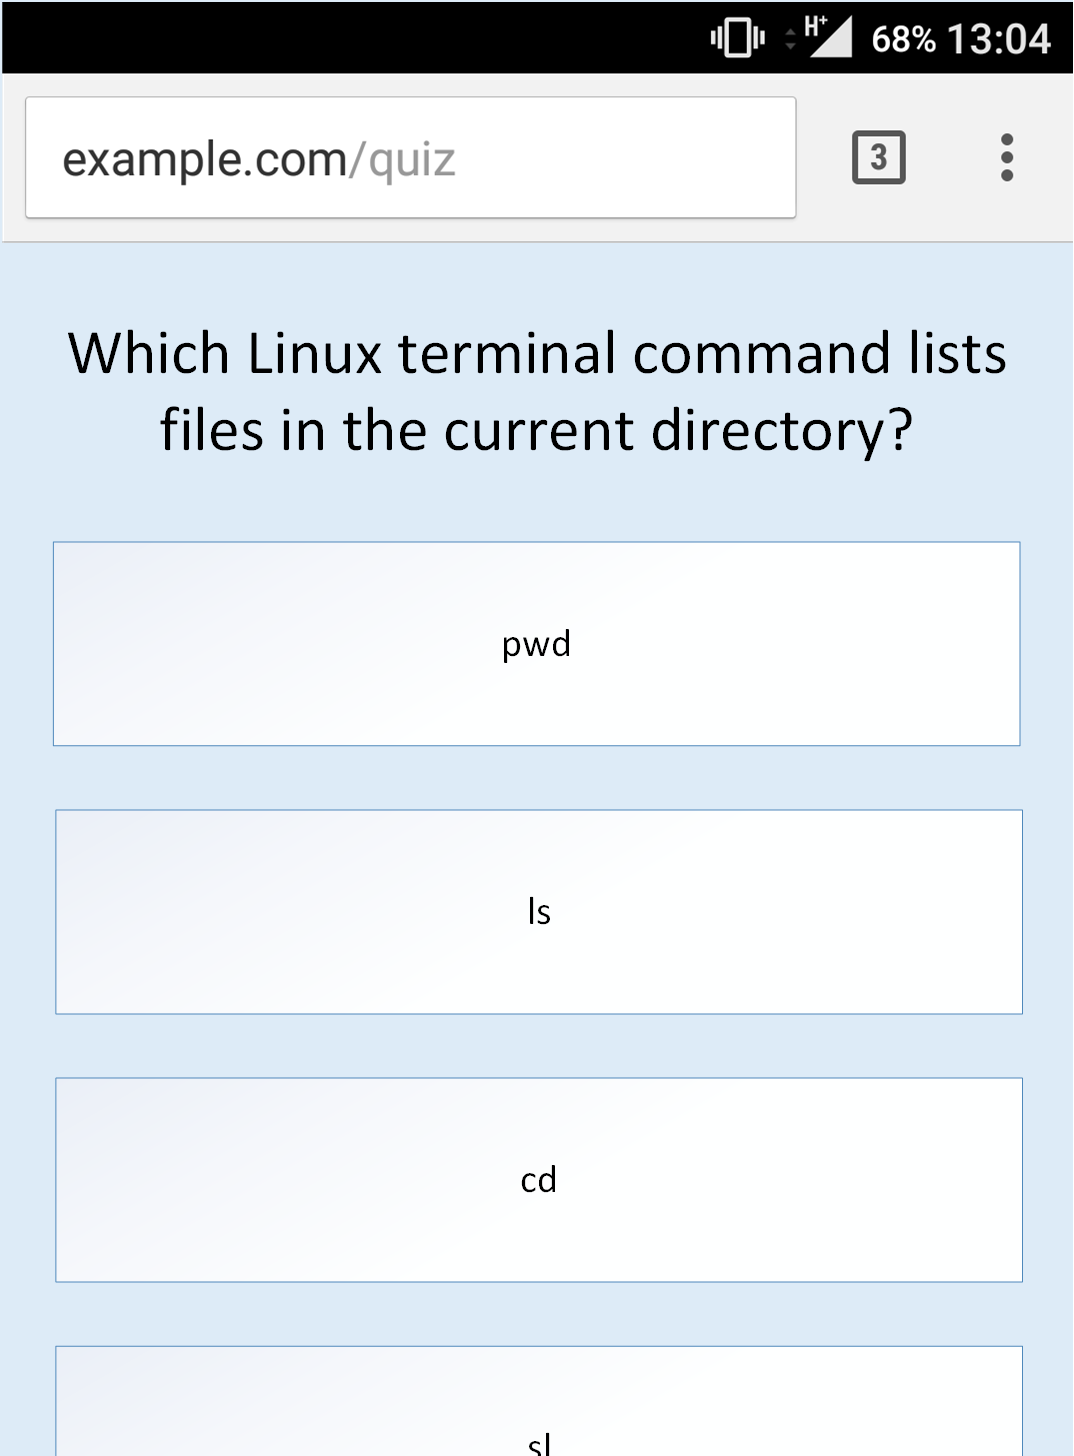
\includegraphics[scale=0.25]{Chapter2/Iter-4/Quiz-Mobile-Cropped}
		\label{fig:quiz-mobile}
	\end{figure}
\end{center}


\subsubsection{Implementation}
It began by configuring pusher, creating an event and writing some basic JavaScript to append to the front page. Some work was done on the admin panel as well, making it only visible to logged in users (the lecturer running the quiz), and adding the functionality for previous and next question buttons. These are buttons that send AJAX requests to quiz controller actions which then trigger the event for WebSockets with the appropriate question data.

Early into the iteration a major flaw with using the WebSockets came up, whilst new content was easy to add to the page, if a new user joined the session late, they would see a blank page/ or the original content of the page that has not yet been removed with JavaScript. To remedy this, the current position in the quiz should be kept track of and the PHP on the page should load the question specified at that position. At the same time, the WebSockets will be running and updating the page from that point onwards in the session. It was decided the best place for keeping track was within the session table, which now has appropriate columns for the position, quiz and if it is running.

Rendering the actual questions calls an action in the question controller, which takes the type of question and the quiz id and position. Using this data it renders one of several available views, one for each type of question like multiple choice or boolean. The views render a simple form showing the question, the possible answers as buttons and a submit button.

For a question to be rendered by default on page load as described above, the page includes the question by rendering the above view. However, it does not know the type of question to render, so it loops over the types and checks if the type of the question is equal to the ones defined earlier in the config file and renders the view if they are the same type. One problem with this is accessing the custom config file. The function to do this was inside the question controller and not the quiz controller. 

Whilst the function could be copied, it was better to create one single helper function that is global to the application. This involved creating a helpers file and adding the function there and then registering the helper function in the composer.json file\cite{laravel-helper-function}.

\subsubsection{Testing}
No testing as the story is not yet complete.
\newpage


\section{Iteration 5 23/03 - 29/04}
\subsection{Story: Admins can login to the backend and run a session with a quiz}
\subsubsection{Analysis - Breakdown of Tasks}
Tasks left over from the previous week:
\begin{itemize}
	\item Form on front page redirects to quiz
	\item Questions rendered as a form
	\item User can submit the form with their answers
	\item Questions need limiting on going above/ below max and min
\end{itemize}
\subsubsection{Design}
\subsubsection{Implementation}
Users still had to connect to the quizzes from the welcome page. A problem with this is that the sessions are being run under the url /quiz/sessionb\_name. This means that submitting a GET or POST form will not work as the url cannot be specified, as the user enters the session key. A solution was to have an input field that took the session key and then used JavaScript to redirect to that session. 

The JavaScript also allowed some client side checking to be done, but there also needed to be server side checks. A custom Middleware class was written to handle the checking of valid session keys. Middleware provide the functionality to filter incoming HTTP requests within controllers\cite{laravel-middleware}. When thr form was submitted, the Middleware function would check the database, and if the requested key was not in the database, would redirect back to the welcome page with an error. Else, it would allow the redirection to the quiz session.

Helper function https://laracasts.com/discuss/channels/general-discussion/best-practices-for-custom-helpers-on-laravel-5?page=2

Issue with Jquery Ajax https://stackoverflow.com/questions/14193469/jquery-is-adding-prevobject-to-array
\subsubsection{Testing}
\subsubsection{Extras}
\newpage

\subsection{Stories Completed}
This iteration and the last have both operated underneath the umbrella of the one story. This is not necessarily accurate as the work that has been completed with this one story covers a multitude of stories. The reason they weren't split up is slightly unclear but part of the reason is the severe overlap between them and some of them being more like functional requirements than areas of work to do. The stories that are now complete:
\begin{itemize}
	\item Multiple different sessions can be run simultaneously
	\item The Admin specifies which question is being run by clicking next/prev question
	\item Sessions can be joined by users via the website
	\item Up to 300 users should be able to join and answer questions (this story is somewhat subjective, but in theory it should scale upwards with no issues)
	\item Users answer the question being displayed by the quiz
\end{itemize}
\newpage

\subsection{Non-Story Work}
\subsubsection{User Page}
A large amount of work was done on the user pages, this was to ensure that admin could view and edit their details including changing their session keys. This work was rather simple and just involved creating the user blade pages, adding the various functions to the controller and model and adding a little bit of functionality to the authentication actions for registering a new user.
\subsubsection{JavaScript Clean Up}
A lot of JavaScript that was being rendered on the page is not used and useless to the project, in fact the libraries are quite large and take up a significant amount of space. Removing these unused libraries, VueJs being the largest, frees up the JavaScript output file considerably, which will increase load times significantly.
\newpage


\section{Iteration 6 30/03 - 05/04}
\subsection{Story: The Admin can show the results of the question in a sensible format e.g. graph}
\subsubsection{Analysis - Breakdown of Tasks}
\begin{itemize}
	\item Save the data
	\item Ensure no users submit twice
	\item Read from that data in the admin panel
	\item Prettify this results tab
\end{itemize}
\subsubsection{Design}
TODO: add design images here of the admin panel
\subsubsection{Implementation}
There was quite a lot of work to do in this story, the first item in particular was the majority of work. At first it was decided that a simple database could be used to store all the responses however it was soon realised that users could probably submit more than once if we don't associate users with a response. The best way to deal with users that don't login is to use the Laravel session cookie to identify them anonymously.

To store all these responses in a database would be quite a lot of data, rather than having say six rows for a question with six answers that just tallies up the answers the actual session name had to be stored with the answer given so it could be changed. This meant that now there would be a row per answer, equalling at worst case 300 rows per question. This was thought to be a bit drastic so an alternative was suggested: to use a CSV file with each row having the user and an answer, with each question being a separate csv file. These would be stored locally under a session folder in the public directory. These files would be created and destroyed during quiz cycle. This method would also be a good for the downloading of answers from another story. 

Ultimately however, trying to write all this data to a csv was too troublesome to be worth it. If a user changed their answer then the entire csv had to be copied with one line changed, editing a single line is not possible with PHP. Therefore it was decided that going back to a database based method would be better, with the idea that at the end of a quiz, all the data would be deleted.

An answers table was created that specified the session, question, user and the answer given. The first three of those were used in a unique composite key to prevent multiple answers from the same users on the same questions in the same session. The model was then written to save this data when data was POST'ed to the /results url. Other functions include those to delete the data when a quiz was ended and various association functions.

To read this data on the front end, an AJAX request was set up from an admin panel button that GETs the same results url which calls an action to render the results data in a JSON format. The results are in a very basic format in a key-value pairs of answer, total number of selections. TODO: maybe talk about this more

This JSON data could then be used in the ChartJS library which was selected to render the results bar chart on the page. TODO: cite http://www.chartjs.org/ and also http://www.chartjs.org/docs also https://www.sitepoint.com/generating-random-color-values/ also https://stackoverflow.com/questions/240660/in-php-how-do-you-change-the-key-of-an-array-element and https://stackoverflow.com/questions/37699485/skip-decimal-points-on-y-axis-in-chartjs
\subsubsection{Testing}
\newpage

\subsection{Story: Users should not be able to submit their own answers by altering the HTML, as they did with Qwizom}
\subsubsection{Analysis - Breakdown of Tasks}
Very few tasks as will be explained in the design subsection:
\begin{itemize}
	\item Add check for empty arrays on frontend
	\item Add check for empty arrays on backend
\end{itemize}
\subsubsection{Implementation}
Thanks to the design of the previous subsection, changing the data meant an empty key was sent if the user tried to change the data submitted to the server. This could be checked in either the JavaScript or PHP end, but it was decided both would be the best for maximum security. 
\subsubsection{Testing}
This is hard to test, as Dusk does not allow the changing of HTML on the page or the possibility to submit false data. User testing might be a good replacement for Dusk tests here.
\newpage

\subsection{Story: The Admin can see what percentage of users connected to the session have answered}
\subsubsection{Analysis - Breakdown of Tasks}
\begin{itemize}
	\item Get total number of responses
	\item Post this number on the page as part of the results form
\end{itemize}
\subsubsection{Design}
This should appear above the results table, possibly as part of the title.
\subsubsection{Implementation}
After attempting to get a number of users connected to the channel it became clear that this number is not readily accessible for public channels. It can be gotten via the Pusher API but implementing that would mean locking some functionality down with Pusher and the long term plan is probably going to involve changing to a Redis based WebSocket system. Therefore this number has just been changed to the total number of responses which should give a good idea to the lecturer of what percentage of users have responded. This was simply added to the title attribute of the chart.
\subsubsection{Testing}
\newpage


\section{Iteration 7 06/04 - 12/04}
\subsection{Story: Site should be mobile responsive}
\subsubsection{Analysis - Breakdown of Tasks}
\begin{itemize}
	\item Create standard media query sizes
	\item Create media query for quiz questions
	\item Media query for welcome page
\end{itemize}
\subsubsection{Design}
A quiz page should look like the design specified in iteration 4.
\subsubsection{Implementation}
Finding the media query sizes was simple, Bootstrap recommends some default sizes for phones, tablets etc. (TODO: cite this https://getbootstrap.com/css/\#grid-media-queries ) It was then a simple task of using the Chrome developer tools to view the page in mobile view and change the various sizes of buttons and titles in the CSS editor to be more mobile friendly.
\subsubsection{Testing}
This is not really possible to test with automated testing, but should be easy to test with users later in the project. Additionally once live the system could be tested with the Google Responsive Test site that gives a score for the usability of a site in mobile view.
\newpage

\subsection{Part Two Re-Design}
Originally planned to be an extension to Microsoft PowerPoint or a similar technology, such as Libre Office, this was determined to be a large amount of work (TODO: cite this). This meant an alternative solution had to be devised or some extra requirements had to be added to the system. An alternative solution was found rather than abandon the idea of having slides within the quizzes. Slideshow programs usually have the ability to render their slides as PDF, a format which is more heavily supported compared to a propriety format such as .pptx provided by Microsoft. If a PDF is uploaded to the application, PHP can be used to turn these PDF slides into images, which can then be rendered on the quiz pages.

This new approach means some changes to the original stories for the second part, here are the revised stories for this part:
\begin{itemize}
	\item (1) The admin creates slides in their preferred editor and exports them as a PDF
	\item (4) The admin can upload these slides to a quiz they have created in the past
	\item (3) The admin can reorder the questions within the quiz to move them around the slides
	\item (2) When this quiz is run, it should render the slides as well as questions in the order specified
\end{itemize}

There are some disadvantages to this however. The main issues is that slide animations are not rendered as separate slides on the PDF. There are extensions for Microsoft PowerPoint that let the slides be rendered with animations occupying separate slides so as to provide a "fake" animation. Another problem is that the slides would have to be uploaded before a lecture as it can take a few minutes to render PDF slides as images. This could be argued as an advantage however, if lecturers upload their slides before a lecture they only need to log in to the application when then want to run them, no need to bother carrying the slides on a memory stick or saving them to their University storage.
\newpage

\subsection{Story: The admin can upload these slides to a quiz they have created in the past}
\subsubsection{Analysis - Breakdown of tasks}
\begin{itemize}
	\item Upload pdf slides
	\item Convert these slides to images
	\item Save references to these slides in the database
	\item Show the slides on the Quiz.show page
\end{itemize}
\subsubsection{Design}
TODO
\subsubsection{Implementation}
To upload the slides, it was done with a standard HTML file input but the backend used techniques native to Laravel: (TODO cite: https://laracasts.com/series/whats-new-in-laravel-5-3/episodes/12). These images are then saved in the /storage/app/public/slides folder. Within this, they are organised into folders named after the session id and then quiz id within those.

These slides are then converted using a library that uses Imagick - (TODO: cite this https://github.com/spatie/pdf-to-image). Whilst saving them, references are also saved to the database. This is so that the images can be referenced quickly later on when displaying an slide or question as database reading is quick. For this functionality, a new table for slides was added to the system, storing the file name, quiz it was associated with and a position. 

The last task involved showing the slides and questions on the Quiz.show page. Seeing as the new story involved reordering them, simply rendering the slides after the questions would not do, it should render them in order of the position. The main problem is that there is no simple SQL query that can select two sets of results and then order them by a common column. The easier solution was to create a PHP function to create an array of all the items in the order wanted. (TODO: Cite this function in appendix, should I explain here or in the appendix?)
\subsubsection{Testing}
\newpage

\subsection{Story: The admin can reorder the questions within the quiz to move them around the slides}
\subsubsection{Analysis - Breakdown of tasks}
\begin{itemize}
	\item Add buttons to reorder questions
	\item This button increases or decreases position of question
	\item It swaps the positions of two questions or a slide and question if required
	\item Add some limits to positioning like not going below 1
\end{itemize}
\subsubsection{Design}
As a minor change to the system, no major design choices were made here. Simple Bootstrap icons can be used for the position changing arrows, which is the only front end change. 
\subsubsection{Implementation}
Main functionality to add was the changing of positions. This was rather simple, adding a simple Route and buttons that triggered the actions associated with the new route. It was decided that the Route would be a POST request rather than GET as technically it is submitting some data, the direction and id of the question. The action it calls simply updates the position in the database after doing some checks of the position it wants to move to. If it is already occupied, it swaps the object at the new position with its current position. This object could be a question or slide.   
\subsubsection{Testing}
\newpage

\subsection{Story: When the quiz is run, it should render the slides as well as question in the order specified}
\subsubsection{Analysis - Breakdown of tasks}
\begin{itemize}
	\item Find the position in the database and decide whether its a slide or question
	\item Render a question like normal
	\item If a slide, render a simple img tag and populate with the image name from the WebSockets
	\item Resize image to fit the page, including for mobile responsive
	\item Render question by default for users joining late
\end{itemize}
\subsubsection{Design}
This should work in much the same way as the questions, in that it will send an Ajax request to a page with the image name and then copy the content of the ajax page into the live page. The content page to Ajax should be pretty simple, a simple container with an img tag. The other tasks are extensions to previously created functions.
\subsubsection{Implementation}
The first task is to determine what is at the position, this involved changing the current function to check if the question at the requested position was null, if it was then it should find a slide at the specified position. As well as the data about the slide or question, it would return a type so that when it was called the system knew what type of content it was to expect. The data was then sent to the WebSockets and another case was added to the JavaScript receiving end for triggering an AJAX call to a slide page. This page would render a simple img tag with the slide specified which is then added to the current page like the questions.

A problem with rendering the images was the files stored within the /storage folder are not publicly accessible, usually only files within the /public folder are. However, there is a simple artisan command to create a symlink from the public folder that points to the storage/app/public folder. TODO add command: php artisan storage:link
\subsubsection{Testing}
\newpage

\section{Iteration 8 13/04 - 19/04}
\subsection{Report writing}
The majority of this iteration was devoted to report writing. Whilst there is still some development to do, the report accounts for 30\% of the final grade and needed to be worked on. There were some small changes to phpdoc and comments added to the code, but no actual functionality was changed. In terms of the report, the first chapter concerning the background had been added. All the iterations documents have also been added into the final report, though they will likely need changing before hand in. There are a lot of TODOs scattered throughout, mostly for citations but also some to check with the project supervisor about certain details. Finally, some content was fleshed out for the testing chapter, giving an overview and descriptions of the technologies.
\newpage

\section{Iteration 9 20/04 - 26/04}
\subsection{Report work}
A lot of report work was completed this last week. This primarily focussed on trying to get through the TODOs scattered throughout the report. It also included adding most of the citations for the system that were noted down during development. The testing and design chapters were also fleshed out far more, and once all this was completed a draft was sent to the project supervisor for some feedback.

\subsection{Security testing}
Five tests were written to test the security of the system. These tested SQL Injection and Cross Site Scripting across the site. Whilst Laravel is supposed to handle much of this it should still be tested to ensure the security of the system. There are only two main places that these attacks can take place, the session search field on the front page of the application, and the question and quiz creation pages in the admin area. The tests proved that Laravel does indeed stop XSS and SQL injection by escaping the inputs. For further information see section \ref{testing:security}.

\subsection{Server setup}
There was some time spent on setting up the server for use in the user tests in the final iteration, the server was provided by the Department of Computer Science. The setup included moving the project onto the server via Git, setting up the MySQL server, and making the site visible to the internet with an htaccess. With this task, help was obtained from two fellow students Stephen James and Max Atkins, and also from the Computer Officer in IMPACS, Alun Jones. This was due to insufficient experience in the area of server setup.

\subsection{Bug fixing}
There was a significant amount of bug fixing in this iteration. The main two were fixing the CSS of the slides in quizzes and multiple selection questions not submitting correctly. 

For the first, a lot of time was spent on trying to write custom CSS for the image tag that would centre it and fill the page. However, there was no need to write any CSS, instead the solution was to add a simple bootstrap container around the image. Whilst the image might be too high for the page, scrolling up and down is not much of a usability problem assuming most slides have blank space at the bottom. This Bootstrap container fixes the image sizing problems that were encountered beforehand, both on a standard desktop and on mobile and tablet devices automatically.

The second major bug fix was to how answers were saved for multiple selection questions. The difference between this and a boolean or multiple choice question is that multiple answers are submitted, and an array was chosen to do this. However, this array was not handled correctly when saving these results. The solution was to create entries of the string versions of the answers joined together, so an answer row would contain the answer of "answer1, answer3". TODO: code snippet of this stuff. Displaying these results did not require much changing except needing to split this string and loop over the items and replacing the "answer1" fields with the actual answer given in the database.
\newpage

\section{Iteration 10 27/04 - 03/05}
Note: This iteration is slightly longer as it includes the half week between where iteration 10 would have ended and the hand in.

\subsection{Story: Admins can then save the results as csv or xml}
\subsubsection{Analysis - breakdown of tasks}
The most convenient way to save these results would be to convert the data to a csv format, as that can be read by many Spreadsheet programs. After some researching, an extension for Laravel was found that could easily create spreadsheets within a Laravel application\cite{laravel-excel}.

There the list of tasks for this story:
\begin{itemize}
	\item Add route, button and an action for this
	\item Install Laravel spreadsheet converter extension
	\item Pass the formatted answer data into the csv creator
\end{itemize}
\subsubsection{Design}
Due to the way the original answer handling was designed, results are only saved for a session and not for quizzes. This means when a new quiz is run, the results are wiped. This means a good place for the download action would be the quiz admin panel, the one next and previous buttons. This would be an ideal place as it means lecturers can hit download before they end the quiz.

The action itself does not seem to fit onto any of the other controllers, and a new one should be created to handle this function. A sessionController would be the best fit as this action falls under a session and not quizzes so would not be sensible in a quiz controller.

The csv format would be in the form of a single sheet with many rows. The first row would be the question, the second row the answers and the third the number of times the answer was chosen. These three rows would then repeat for each question, so a three question quiz would contain nine rows.
\subsubsection{Implementation}
Setting up the new route, button and controller was a quick task. Artisan (TODO have i mentioned artisan before?) was used to generate the new controller and then all that needed manually doing was adding a route to the web routing file and creating a new button on the admin panel to call this route.

Installing the extension was done with Composer which installed it under the vendor/ folder. It was then added as a Facade\cite{laravel-facades} which allow the quick use and access to the functions it contained. The extension took an array of data and turned that into a spreadsheet of the type specified, in this case a csv. The array is looped over and each item in the array is a row in the sheet. If an item of the array is an arrays itself, then each item within these sub arrays would be a cell within the row. This means the sheet is built from an array of arrays. 

Formatting the arrays was the primary task here. First all the questions from the session were selected, then looped over. Within this loop the question was added as the first row. Then all the answers associated with that question needed to be added. Getting them from the database used a simple Eloquent query. Two arrays needed to be created from this data, an array of the answer text and an array of the number of times these options were submitted. The total times these were submitted had not been calculated so this was done first, looping over the answers and counting the times an answer was given by creating a new array of the answers and times clicked in a key=>value pairing. This array of answer=>answeredNumberTimes could then be looped over and the each key added to the first array, and the values to the second array for the two rows.

The problem here was that the answer text in the database is stored as "answer1" rather than what the student actually clicked. This meant that these answers had to be changed, this was accomplished by using the answer value, like "answer1", as the key in the current question variable and adding this value to a new "keys" array. Another problem was the way multi selection questions were stored, such as "answer1, answer2". This meant adding another extra step to break the string into an array and replacing them with the actual answer values and recombining them into a single string.

(TODO add code snippet and image of a csv)
\subsubsection{Testing}
TODO
\newpage

\subsection{Extra implemenation based on feedback from admin user tester}
An admin user effectively tested the application whilst using the system to build a quiz that would be used in the user testing. During this, some feedback was received about the application which could be worked on to improve it in small ways.
\subsubsection{Quiz control buttons should be greyed out}
The next and previous buttons on the quiz were changed so that they should be greyed out if the quiz was at the start or end of the quiz. To disable them the "diabled" HTML attribute was added to the buttons. The position and total number of items in the quiz were passed to the page from the controller and could be used to determine whether or not the buttons should be disabled. For these to be disabled when the page loads, some embedded PHP was used to render the buttons with disabled if needed. When the quiz was running, JavaScript was used to add and remove the disabled attribute whenever next or previous was pressed.
\subsubsection{Question creation true/ false changes}
Some JavaScript was used to change the question creation and question edit pages. It was needed for true/ false questions which should be submitted with answer1 as 'True', and answer2 as 'False', with the other fields left blank. The other fields would be ignored when the question was rendered, but allowing them to be filled in could be confusing. So JavaScript was used to hide the other fields, fill the first two with 'True' and 'False', and disable the fields so they could not be edited. This was actually part of the original design for the question creator but was left due to more pressing tasks such as the running of quizzes.
\subsubsection{Cancel button on question edit pages}
Finally, the tester asked if a cancel button could be added, as pressing the back button would work but having a button would probably be better for the users. This was simple a back button placed at the bottom of the edit page.

\subsection{Bugs}
Various bugs were fixed in this final iteration after being found by the admin user. One was a bug concerning the upload time of slides, which took long enough for the PHP execution time to be exceeded. Whilst normally this would require a change to the php.ini file, this was not easily accessible on the server, so a call to the php function, set\_time\_limit() was made to increase this past the default for the function in question. This was probably a better solution due to it only increasing the limit for the one function, whereas changing the times in the ini file would change the whole system and possibly lead to unintentional side effects.

Another small bug was a "LogicException" found by going to an incorrect url, which is not the standard 404 thrown by an incorrect url. This was caused by a route which had no defined action in the router, something left over from an earlier iteration that ought to have been deleted.

\subsection{User testing}
Used the system in a first year workshop to gather some module feedback for the lecturer and to test the system with real users.

\subsection{Report writing}
A lot of report work in this final iteration, including the restructuring of the iteration and design chapters, writing the design, evaluation, appendices, and generally editing the whole document based on feedback from proof readers.
\newpage
\chapter{Testing}

\section{Overview}
At the start of the project, testing was to use two practices from Agile. These were Test Driven Development and Continuous Integration (CI). Whilst these two practices both failed due to a mixture of reasons as described in the Iterations chapter, testing was still performed within each iteration. Rather than go over the tests made each week within the previous chapter, this section will summarise the tests. Overall there were x tests (TODO: fill in once development finished) that test the overall functionality of the system. Unit tests were dropped for a number of reasons in favour of application tests.

Unit testing suits a situation where more of the base code is written by the developer, in this case the majority of the code is built on a pretested framework. Testing the final implementation would fit better than trying to test if a view is rendered by a controller correctly. Application tests can also be used to test the stories, meaning that they can give a much clearer indication of whether a story is complete and whether the customer will be happy.

Unit testing also takes up a lot of time if done as well as application testing which would have affected the final product and dropping it was a necessary exchange to save development time.

\section{Application testing}
TODO: screenshot final output of all tests. Also could list all tests somewhere in appendix?
To do application tests, a testing framework called Laravel Dusk was used, which is the default testing framework provided with Laravel 5.4\cite{dusk}\cite{dusk-desc}. It runs the tests within a Chrome instance by running a standalone server which then calls the Chrome application installed on the machine that the tests are being run on. The advantages of running tests like this rather than say executing PHP on the server and reading a virtual DOM is that this allows JavaScript on the page to be evaluated and executed. JavaScript is vital to many of the components of the application so if it was not usable within tests, many parts of the system would have to be ignored within the tests.

These tests test the application as whole, rather than individual bits of code. This allows the tests to be written with the original requirements, the stories, in mind and so makes these tests a good way to evaluate the application at the end of its development. Tests were organised by story, as these provided an area of the application that needed to be checked, which makes them more human readable for any future development.

Tests use a test database rather than the production one to ensure the integrity of data on the production system. This test database is left intentionally empty when, with each test performing a migration for the test. Within each test the database is populated with relevant data using a number of database factories. These factories allow the easy and quick creation of any data needed within the test, though using a normal Model to input data would also still work. At the end of each test, the database is rolled back for the next test to run, leaving an empty database for a new migration and data.

Database transactions could have been used instead, which use a pre migrated database and then any data input during each test is deleted at the end of the test. Whilst the test db could be migrated before any tests were run to allow the use of transactions, this would mean than any future changes to the migration files would mean that the developer would have to remember to re-migrate the test database as well. Doing a migration for every test might be somewhat resource intensive, but it allows the tests to be written and run completely standalone from each other with no need to tie into any earlier setup functions. 

\subsection{Limitations of dusk}
Various problems
Also cucumber or something?
Dusk cant do WebSockets for some reason, assume blocking communication?
Dusk cannot see inside Canvas tags
Dusk selectors are rubbish, sometimes by text, sometimes id but never returns a collection, always the first item it sees
Lots of code repetition for moi
Pauses

\section{Security testing}
One story specifically concerns security: Users should not be able to submit their own answers by altering the HTML, as they did with Qwizdom. The tests for this however are not that easy to do within the confines of Dusk due to the nature of the framework. The framework is concerned with user facing application tests and has no ability to change the DOM of the page or send custom POST requests to the server. This means that this story is better tested in the user testing section.

Other aspects of security can be checked however, being a web application there are a number of well known attack types including SQL injection, cross site scripting (XSS) and cross site request forgery (CSRF) attacks. These tests are located in SecurityTest.php. There are five tests that test both SQL Injection and XSS attacks. SQL injection attacks involves attackers trying to execute their own SQL code on the server, thereby giving them access to the system or to try and damage the system by say dropping some tables. XSS attacks are when attackers attempt to inject thier own JavaScript into the system that may be run on another users page. Typically this would include injecting a script tag with malicioud code into the database that would then be executed when written to the page by another user viewing a page. (TODO: cite these?) 

For the SQL injection tests, a string that tries to insert a new database extry is used:
\begin{verbatim}
	"INSERT INTO `quizzes` 
		(`name`, `desc`, `user_id`, `created_at`, `updated_at`) 
		VALUES ('SQL Injection', 'this is an attack', '1', now(), now());"
\end{verbatim}
And for the XSS attacks it tries to add a script tag with an alert:
\begin{verbatim}
	<script>alert('hey xss');</script>
\end{verbatim} 

There are two main places that these attacks can be carried out. The first is on the front page, the session search field could be used to insert malicious data. Though nothing is saved from this input, it does query the database, which means it could be subject to an SQL injection attack. If the search returned the original search query, then it could be used to embed some javascript, and if the search was then linkable (i.e. in the URL parameters), it could be sent on to other users. The other place that these two attacks can be carried out are on the admin area, in the quiz and quetion creation pages where SQL or XSS code could be added to the body of the various quiz and question fields.

For SQL injection attacks, the easiest way to check that this data has not been added is to look for the record in the quizzes table. With the XSS attack, the page source can be searched for the script tag. Laravel copes with these attacks by default by escaping the inputs\cite{laravel-web-attacks}. With SQL, the entire string is quoted and not seen as an actual SQL command. With the XSS the HTML tags are escaped in a similar fashion, the \textless and \textgreater symbols are turned into \&lt; and \&gt; which are not rendered as HTML when written to the page.

The tests prove that the system works as intended and these two attack types are not possible. Cross site request forgery attacks are another form of attack but harder to test as they rely on the browsers weaknesses and come from another website. Dusk cannot simulate this sort of environment. However, for forms to be submitted within the system a CSRF token has to be submitted with the form. This token is compared to the user session to ensure they are the ones submitting this data, not a third party site. Laravel forces forms to contain this token, ensuring this attack cannot take place. 

\section{User testing}
TODO

\section{Stress testing}
Though there are a number of tools out there to do exactly that, there was no time to set up and any official stress testing. However, the user tests within the lecture helped a give a good idea of the stress the system could take. Like many sites though, the application was mostly restricted by its server setup rather than by its design. (TODO: prove after user testing)

\section{Automated testing}
Whilst CI was abandoned early on into the development of the application, the Dusk tests are easy to run and automatically execute within a browser if the appropriate browser drivers are available. This means that it should not be too hard to integrate these tests into a CI tool if required in any future development.


TODO: Stuff to talk about:

comprehensiveness of testing incl potential of using bdd and cucumber in future

edge cases? how did we manage those = (user and application)
\chapter{Evaluation}
\begin{itemize}
   \item Were the requirements correctly identified? 
   \item Were the design decisions correct?
   \item Could a more suitable set of tools have been chosen?
   \item How well did the software meet the needs of those who were expecting to use it?
   \item How well were any other project aims achieved?
   \item If you were starting again, what would you do differently?
\end{itemize}
\section{Story/ requirements comparison}
For the final list of stories see appendix \ref{appendix:final-stories}. When looking at the final application and the final stories, they can all be argued as being completed with the exception of stories 7, 9 and 12. 

Concerning story 7, whilst technically the application only supports up to a hundred users simulataneously, this is not throttled by the application. But instead is due to the WebSockets provider Pusher, which for free use is limited at a hundred users. If the system were to go live, then this would be replaced by using an in house Redis server, or by paying Pusher for more slots. These would be able to meet this upper capacity and therefore meet the story. For story 9, a percentage of answers was decided to be too hard to do without relying too much on the WebSocket server being used, which as mentioned above could be changed therefore a simpler solution was added, just giving the number of answers submitted. This number would give a rough estimate of the percentage, as if the lecturer knew the class size, they could compare it to the number answered. It was important to not rely on Pusher and instead offer an alternative solution that did not quite meet the story.

As for the final story that was not completed, 12, the downloading of stories was done in the last iteration. It was decided that the reuploading of these to view on the application would have taken too long given how much other work was yet to be completed. Additionally, due to the download being a csv rather than the other potential format (XML), if the lecturer wished to view the results in a more graphical view, their preffered spreadsheet can easily be used to create graphs of the data. Whilst this is more work for the lecturer, it seemed like a minor issue and one worth causing if it meant more time for writing the report.

Of course, there were significant difference between the initial list of stories, \ref{appendix:initial-stories}, and the final list. A couple of new ones were added, such as number 14 and 15 on the final list. However, all the stories for part two were changed. The reasons for these changes have already been explained but it is obviously different from the initial set of stories. However, the redesign and production of new stories fills the same functionality as originally specified and therefore it can be argued that the original specifications are still met.

\section{Methodology}
I am very happy with the the methodology used. XP's main strength is its adaptability and the first thing to do was adapt a set its practices to fit the needs of the project. This was very beneficial as some practices were not relevant and would have not worked or even hindered the development. As development progressed, some of the practices had to be further adapted, such as dropping test driven development, allowing even more flexibility to the way I worked.

I particularly liked working to stories and in iterations. The iterations allowed small bits of working functionality to be written on a weekly basis. They were particularly useful in that they enforced small bits of design, implementation and testing each week, meaning there was a good mix of things to do. But most importantly, the iterations helped adapt to change. The best example is the part two redesign, which was originally planned to include a lot of work, two or three iterations worth, but instead came down to less than a full iteration of work. The iteration also included the creation of a review document at the end. This was used to evaluate the work done and the methodology itself, such as deciding that TDD should be dropped.

There were some problems though, the design and testing sections sometimes suffered within the iterations. This was because I was more interesting in getting the implementation done. Its not to say that design and testing didn't happen when they were supposed to, its just that occasionally it had to be done the following iteration.

Another major problem is that due to a lack of overall design at the start, as encouraged by the use of XP, there was some redesigning and reimplementation happening throughout. This effectively meant that some of the work could have been avoided if it had been designed from the ground up. An upfront design might also have led to an overall better design, rather than what sometimes feels like lots of small bits of functionality tied together. On the flip side though, it might have caused there to be too much work, seeing as without the iterations part two might have been designed in a way similar to the original proposals.
\section{Tools and technologies}
Laravel, Dusk, Websockets, Javascripty stuff, Chrome? Editor? --Better tools? Diary, Trello, Git
\section{User testing evaluation}
\section{Summary}
% add any additional chapters here

\setemptyheader
\addcontentsline{toc}{chapter}{Appendices}
\chapter*{Appendices}

\pagebreak

% start the appendix - sets up different numbering
\fancypagestyle{plain}{%
%\fancyhf{} % clear all header and footer fields
\fancyhead[L]{\textsl{Appendix\ \thechapter}}
\fancyhead[R]{\textsl{\leftmark}}}

\appendix
\fancyhead[L]{\textsl{Appendix\ \thechapter}}
\fancyhead[R]{\textsl{\leftmark}}
\fancyhead[C]{}
\fancyfoot[C]{\thepage}
\renewcommand{\headrulewidth}{0.4pt}
\renewcommand{\chaptermark}[1]{\markboth{#1}{}}

\fancyhead[L]{\textsl{Appendix\ \thechapter}}
\fancyhead[R]{\textsl{\leftmark}}
\fancyfoot[C]{{\thepage} of \pageref{LastPage}}

% include any appendices here
\chapter{Third-Party Code and Libraries}
TODO:
Laravel
Pusher
EchoJS
JQuery
ChartJS

\chapter{Ethics Submission}
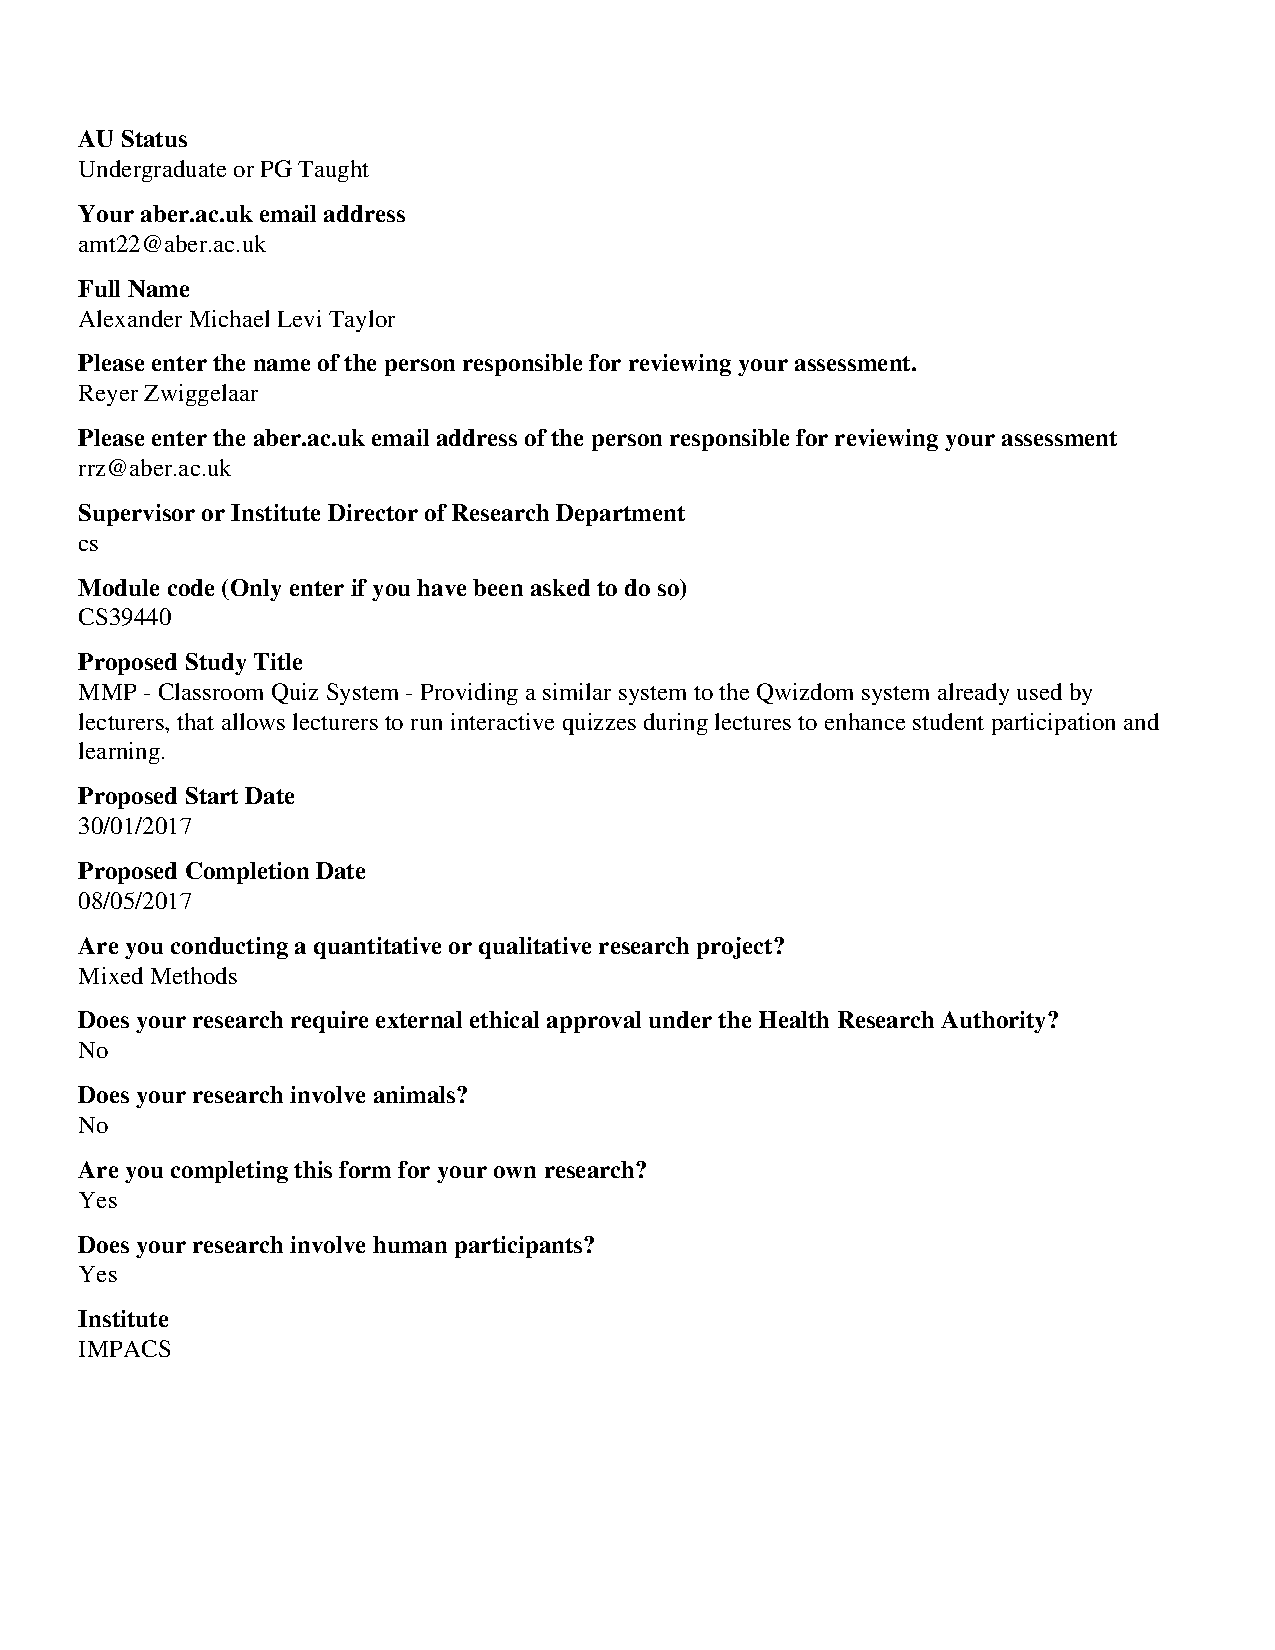
\includepdf[pages={1}]{Appendix2/ethics-submission.pdf}

\chapter{Code Examples}


\chapter{User survey results}
\label{appendix:user-results}
For all the raw results, please contact amt22@aber.ac.uk.
\chapter{Desktop}
\chapter{Mobile}
\chapter{Comments} 
\chapter{Lecturer results}

\fancypagestyle{plain}{%
   \fancyhead{} %[C]{Annotated Bibliography}
   \fancyfoot[C]{{\thepage} of \pageref{LastPage}} % except the center
   \renewcommand{\headrulewidth}{0pt}
   \renewcommand{\footrulewidth}{0pt}
}

\setemptyheader

\nocite{*} % include everything from the bibliography, irrespective of whether it has been referenced.

% the following line is included so that the bibliography is also shown in the table of contents. There is the possibility that this is added to the previous page for the bibliography. To address this, a newline is added so that it appears on the first page for the bibliography. 
\addcontentsline{toc}{chapter}{Annotated Bibliography} % Adds References to contents page

%
% example of including an annotated bibliography. The current style is an author date one. If you want to change, comment out the line and uncomment the subsequent line. You should also modify the packages included at the top (see the notes earlier in the file) and then trash your aux files and re-run. 
%\bibliographystyle{authordate2annot}
\bibliographystyle{IEEEannotU}
\renewcommand{\bibname}{Annotated Bibliography} 

\bibliography{References/references} % References file

\end{document}
